\selectlanguage{ngerman}%
\frenchspacing%
\begin{ledgroupsized}[r]{120mm}%
\footnotesize%
\pstart%
\noindent\textbf{Überlieferung:}%
\pend%
\end{ledgroupsized}%
\begin{ledgroupsized}[r]{114mm}%
\footnotesize%
\pstart%
\parindent -6mm%
\makebox[6mm][l]{\textit{L}}%
Aufzeichnung:
LH~XXXV~11,\;14 Bl.\;35. 
Ein Zettel (7,5\;x\;11~cm);
Ränder tlw. beschnitten.
Eine Seite auf Bl.\;35\,v\textsuperscript{o}.
Bl.\;35\,r\textsuperscript{o} ist unbeschrieben.
\pend
\end{ledgroupsized}
\vspace{5mm}
\begin{ledgroup}
\footnotesize
\pstart
\noindent%
\textbf{Datierungsgründe:}
Die Datierung der Aufzeichnung N.\;\ref{58950} beruht %
auf inhaltlichen Betrachtungen.
Siehe die ausführliche Begründung auf S.\;\pageref{58950_dat}.
\pend 
\end{ledgroup}
\selectlanguage{latin}
\frenchspacing
\vspace{8mm}
\pstart%
\normalsize%
\noindent%
\edtext{%
\lbrack%
\href{\Scan{LH_35_11_14_035v}}%
{35\,v\textsuperscript{o}}%
\rbrack\ %
Supersunt adhuc quaedam explicanda,%
\indexS{explicandum}%
}{%
\lemma{\lbrack\href{\Scan{LH_35_11_14_035v}}{35\,v\textsuperscript{o}}\rbrack}%
\Bfootnote{%
\textit{(1)}~Difficultas\indexS{difficultas}
\textit{(2)}~Supersunt adhuc quaedam explicanda,%
~\textit{L}}
}
ut quid fiat
si corpora,%
\indexS{corpora concurrentia}
globi%
\indexS{globus}
exempli causa,
concurrant,
qui simul gyrentur circa sua centra.%
\indexS{gyratio circa centrum}%
\indexS{corpus gyrans circa suum centrum}
Et videndum,
an concursus%
\indexS{concursus corporum}
idem
\edtext{%
praestent quoad progressus,%
\indexS{progressus post concursum}
sive%
}{%
\lemma{praestent}\Bfootnote{%
\textit{(1)}~, sive
\textit{(2)}~quoad progressus, sive%
~\textit{L}}}
gyrentur sive non,
gyris tantum in gyros%
\indexS{gyrus transfusus in gyrum}
\edtext{%
transfusis.
Sed hoc intelligendum 
arbit\lbrack r\rbrack or
de concursibus
centricis,%
\indexS{concursus centricus}
\edlabel{LH_35_11_14_035_035v_gyros-1}%
nam si sint eccentrici%
\indexS{concursus eccentricus}
fieri potest ut gyri%
\indexS{gyrus transfusus in progressum}
aliquid faciant in progressus,%
\indexS{progressus post concursum}
quoniam gyri%
\indexS{gyrus ortus e progressu eccentrico}
etiam ex progressibus eccentricis%
\indexS{progressus eccentricus}
sunt orti%
}{%
\lemma{transfusis}\Bfootnote{%
\textit{(1)}~, quanquam gyri aliqui ex progressus\lbrack\textit{!}\rbrack\ sin
\textit{(2)}~. Sed hoc intelligendum
\bars{arbitor \textit{ändert Hrsg.}} de
\textit{(a)}~gyris
\textit{(b)}~concursibus centricis, %
\lbrack...\rbrack\ sunt orti%
~\textit{L}}}
atque adeo eos possunt reproducere.%
\edlabel{LH_35_11_14_035_035v_gyros-2}%
\pend%
\pstart%
\edlabel{LH_35_11_14_035_035v_tang-1}%
Videndum et
quid fiat in singulari quadam concursuum obliquitate.%
\indexS{obliquitas concursus}
In concursibus%
\indexS{concursus corporum}
quidem \textit{A}, \textit{B}, \textit{C} res videtur absoluta,%
\indexS{res absoluta}
sed in \textit{D}, \textit{E}, \textit{F} non aeque.
An dicemus
\edtext{%
in \textit{D} ictum%
\indexS{ictus perpendicularis plano}%
}{%
\lemma{in \textit{D}}\Bfootnote{%
\textit{(1)}~concursum
\textit{(2)}~ictum%
~\textit{L}}}
fieri in perpendiculari
ad planum;%
\indexS{planum}
in \textit{E} vero quaeritur
ictusne%
\indexS{ictus normalis bisecanti}
fieri intelligatur ad \textit{lm},
quae normalis bisecanti%
\indexS{bisecans angulum}
angulum ipsius \textit{r},
an ad \textit{np}
quae normalis
\edtext{%
bisecanti%
\indexS{bisecans angulum}
angulum ipsius \textit{s},%
}{%
\lemma{bisecanti}%
\Bfootnote{%
\textit{(1)}~ipsius %
\textit{(2)}~angulum ipsius \textit{s},%
~\textit{L}%
}}
an utrumque conjungendum,
et quomodo.
Denique in \textit{F},
ubi \textit{t} in vertice%
\indexS{vertex}
habet tangentes,%
\indexS{tangens in vertice}
quaeritur
an omnes illi tangentes%
\indexS{tangentes conjungendae}
conjungendae.%
\edlabel{LH_35_11_14_035_035v_tang-2}%
\pend%
\vspace{1.75em}
\centerline{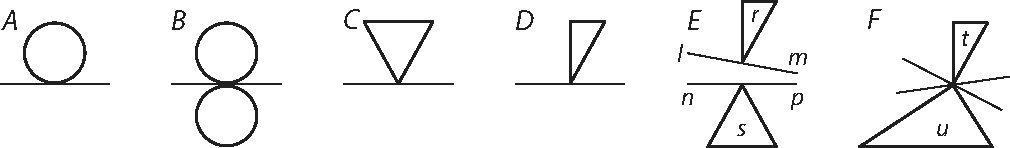
\includegraphics[width=0.96\textwidth]{gesamttex/edit_VIII-4/images/LH_35_11_14_035_d_035v.pdf}}
\vspace{0.00em}
\centerline{\lbrack\textit{Fig.\:1}\rbrack}
\newpage%
\vspace*{1.0em}%
\pstart%
\noindent%
\centering%
*    *    *
\pend%
\vspace{2.0em}%
\begin{ledgroup}
\footnotesize
\pstart
\noindent%
\textls{Ausführliche Datierungsgründe:}%
\pagelabel{58950_dat}
Die undatierte Aufzeichnung N.\;\ref{58950} ist auf einem Textträger überliefert, der weder Spuren eines Wasserzeichens aufweist noch äußere datierungsrelevante Anhaltspunkte bietet.
Inhaltliche Überlegungen ermöglichen jedoch wenigstens eine grobe chronologische Einordnung des Textes:
\pend%
\pstart%

Die Aufzeichnung wirft zwei verschiedene Fragen auf, welche eine bemerkenswerte Verwandschaft mit der Thematik des exzentrischen Stoßes aufweisen:
Die erste ist, ob die Bewegung des Schwerpunkts (\textit{progressus}) zusammenstoßender Kugeln sich ändert, wenn diese sich um ihren jeweiligen Mittelpunkt drehen;
bei der zweiten Frage handelt es sich ansatzweise um die kinematischen Folgen des schiefen Stoßes.
Bereits der Anfangssatz \textit{Supersunt adhuc quaedam explicanda ...} legt nahe, dass N.\;\ref{58950} die Fortsetzung eines mit der Stoßlehre befassten Textes ist.
Zwar lässt sich nach heutigem Wissensstand nicht eindeutig ermitteln, woran die Aufzeichnung N.\;\ref{58950} unmittelbar anknüpft.
Aber die den ersten Textteil abschließende Feststellung \textendash\ bei exzentrisch zusammenstoßenden Körpern wirkten sich ihre Drehungen zweifelsohne auf die Bewegung des Schwerpunkts aus, weil %
die Drehungen ohnehin aus der Bewegung des Schwerpunkts entstanden seien und diese "reproduzieren" könnten (\refpassage{LH_35_11_14_035_035v_gyros-1}{LH_35_11_14_035_035v_gyros-2}) \textendash\ bezeugt wohl Leibnizens ausgeprägtes Verständnis des exzentischen Stoßes.
\pend%
\pstart%
Mit der Kinematik exzentrisch zusammenstoßender Körper, sowie zum Teil mit der des schiefen Stoßes, waren bereits Texte aus den 1680er Jahren befasst (siehe etwa \textit{LSB} VIII,\;3 N.\;63 und N.\;64).\cite{01399}\cite{01400}
Die Lehre vom exzentrischen Stoß entwickelte sich aber vorwiegend in den frühen 1690er Jahren im Anschluss an die Stoßlehre der \textit{Dynamica},\cite{01354} wie zahlreiche Texte im vorliegenden Band zeigen (u.\,a. die Aufzeichnung \textit{De impulsu eccentrico} N.\;\ref{60300} sowie die \textit{Schedae de impulsu eccentrico} N.\;\ref{sdie_intro} und der Textkomplex  \textit{Casus eccentrici concursus simplicissimus} N.\;\ref{cecs_intro}).
Demnach ist anzunehmen, dass auch die Aufzeichnung N.\;\ref{58950} etwa zur gleichen Zeit wie diese Texte enstand, wahrscheinlich nach den von Leibniz eigenhändig auf den 31.\;Oktober\,/\,10.\;November 1690 datierten \textit{Schedae de impulsu eccentrico} N.\;\ref{58940} und N.\;\ref{58939}, in denen die Kinematik des exzentrischen Stoßes besonders umfassend und systematisch behandelt wird.
Eine frühere Entstehung ist möglich;
es ist aber unwahrscheinlich, dass die Aufzeichnung N.\;\ref{58950} vor der Aufzeichnung N.\;\ref{60300} abgefasst wurde, da die Kinematik des exzentrischen Stoßes vor Leibnizens Rückkehr aus Italien\indexO{Italien} noch erheblichen Schwankungen unterlag (siehe die ausführlichen Datierungsgründe zu N.\;\ref{60300}, S.\pageref{LH_37_05_044_datierung}).
\pend%
\pstart%
Ein eindeutiger Terminus ante quem der Datierung lässt sich für die Notiz N.\;\ref{58950} zum Redaktionsschluss nicht angeben.
\pend 
\end{ledgroup}
\selectlanguage{latin}%
\frenchspacing%
\normalsize%
